\subsubsection{ClientController}

\textbf{NetworkIntentService}

\paragraph{Database}

Die folgenden Service Klassen stellen die grundlegenden Funktionen zur Verfügung, mit welchen auf die Daten der in den Innenklassen von FeedReaderContract definierten Datenbanken zugegriffen werden kann. Dabei können Daten hinzugefügt (insert), gelesen (read), gelöscht (delete) und verändert (update) werden.
Weitere Details dazu, wie die jeweilige Datenbanken aufgebaut sind, finden sie in FeedEntryAllocation, FeedEntryAppointment, FeedEntryGroup und FeedEntryUser.

\textbf{ServiceAllocation}
\begin{figure}[H]
	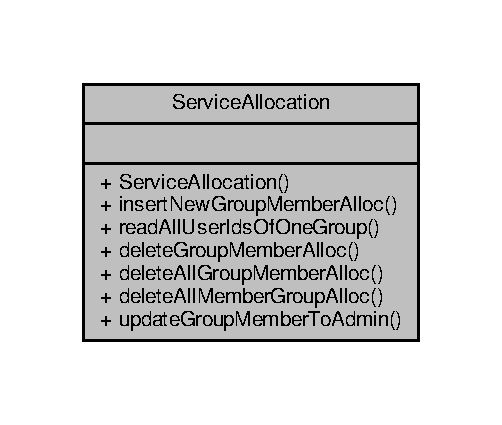
\includegraphics[scale = 1]{res/umlClasses/service_allocation__coll__graph.pdf} 
	\centering
\end{figure}
In der Datenbank auf die ServiceAllocation zugreift, wird die Verbindung zwischen Gruppen und Gruppenmitgliedern bzw. Administratoren gespeichert. 
Sobald ein Mitglied einer Gruppe hinzugefügt oder aus einer Gruppe entfernt werden soll, wird entweder eine Verbindung erstellt oder gelöscht. 
Um in der App dem Benutzer alle seine Gruppenmitglieder anzeigen zu können, müssen alle UserId's mit derselben GruppenId zurückgegeben werden, um anschließend die dazugehörigen Benutzernamen zu visualisieren.
Update wird bei diesem Service nur benötigt, sobald ein normales Gruppenmitglied zum Gruppenadministrator gemacht werden soll und sich die Administratorvariable ändert.
	
\textbf{ServiceAppointment}
\begin{figure}[H]
	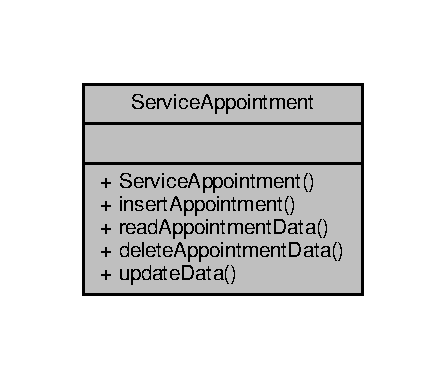
\includegraphics[scale = 1]{res/umlClasses/service_appointment__coll__graph.pdf}
	\centering
\end{figure}
In der Datenbank auf die ServiceAppointment zugreift, wird zu jeder Gruppe das aktuelle Treffen gespeichert und verändert, sobald ein neues existiert. 
Sollte die Gruppe gelöscht werden, so wird auch das Treffen aus der Datenbank entfernt.

\textbf{ServiceGroup}
\begin{figure}[H]
	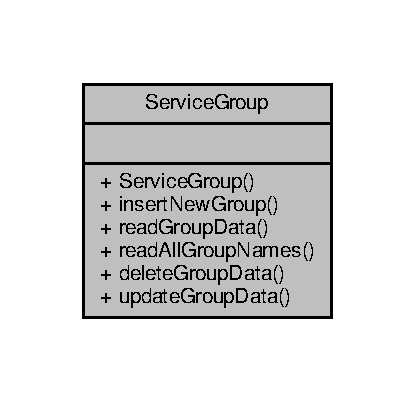
\includegraphics[scale = 1]{res/umlClasses/service_group__coll__graph.pdf}
	\centering
\end{figure}
In der Datenbank auf die ServiceGroup zugreift, werden die Gruppen gespeichert und ob der aktuelle Nutzer der Go-App für diese spezielle Gruppe seinen Go-Button aktiviert hat oder nicht. Sobald sich dieser Zustand ändert, wird das auch sofort in der Datenbank angepasst. Dasselbe gilt, wenn der Gruppenname nachträglich nochmal verändert wird.

\textbf{ServiceUser}
\begin{figure}[H]
	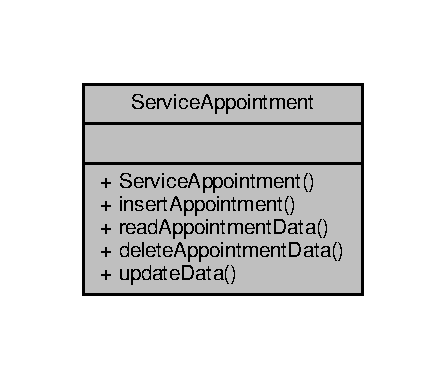
\includegraphics[scale = 1]{res/umlClasses/service_appointment__coll__graph.pdf}
	\centering
\end{figure}
In der Datenbank auf die ServiceUser zugreift ist der Name und die zuletzt bekannte Position des Benutzers gespeichert, welche bei neuen Informationen angepasst werden. 
Ein Benutzer wird nur aus dieser Datenbank gelöscht, wenn er in keiner einzigen Gruppe mehr mit dem aktuellen User ist.
Sobald der aktuelle Benutzer mit einem Gruppenmitglied in einer Gruppe ist, wird dieses auch auf dem Endgerät gespeichert.


\paragraph{ObjectStructure}

In Account- und GroupHandler werden allgemeine Funktionen definiert, die nicht selbst vom GroupClient oder von Unterklassen von UserComponent ausgeführt werden können, sondern eine übergeordnete Position benötigen.

\textbf{AccountHandler}
\begin{figure}[H]
	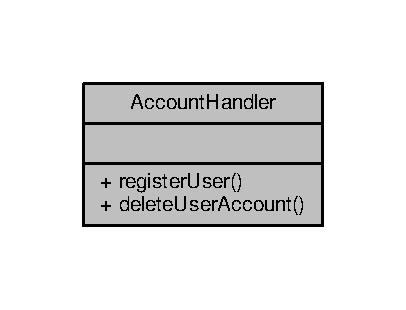
\includegraphics[scale = 1]{res/umlClasses/account_handler__coll__graph.pdf}
	\centering
\end{figure}
Die AccountHandler Klasse handelt dabei nur Benutzer registrieren und Benutzer löschen ab.
Beim Registrieren wird der Benutzer zunächst als SimpleUser Objekt angelegt, welches dann zur Laufzeit grundlegende Informationen bereit hält, um den aktuellen Benutzer in den Gruppen von den anderen Gruppenmitgliedern unterscheiden zu können. Im Gegensatz zum Client wird dieser dann zusammen mit seiner DeviceId gespeichert, so dass jedes Mobiltelefon nur einen Benutzer unterstützt.
Beim löschen des aktuellen Nutzers wird dieser vom Client als auch vom Server mit samt seiner DeviceId entfernt. Es werden keine Informationen über den Benutzer nach Löschen seines Accounts gespeichert.

\textbf{GroupHandler}
\begin{figure}[H]
	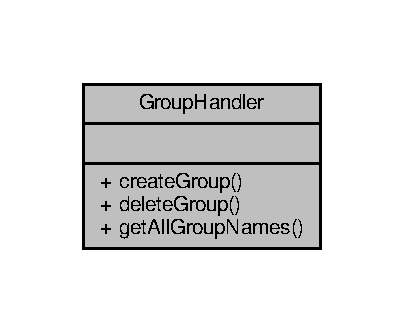
\includegraphics[scale = 1]{res/umlClasses/group_handler__coll__graph.pdf}
	\centering
\end{figure}
Der GroupHandler handelt im Prinzip dieselben Funktionen wie der AccountHandler ab. Wird eine neue Gruppe erstellt, so wird diese auf dem Server als auch auf dem Client angelegt. Hinzu kommt, dass der Benutzer, welcher die Gruppe erstellt hat automatisch zum Administrator dieser wird.
Beim löschen werden alle Mitglieder entfernt und dann die Gruppe selbst vom Client und Server gelöscht.
